\documentclass[border=10pt]{standalone}
\usepackage{tikz}

\usepackage{amssymb} %maths
\usepackage{amsmath} %maths
\usepackage[utf8]{inputenc} %utile pour taper directement les caractères accentués

\begin{document}

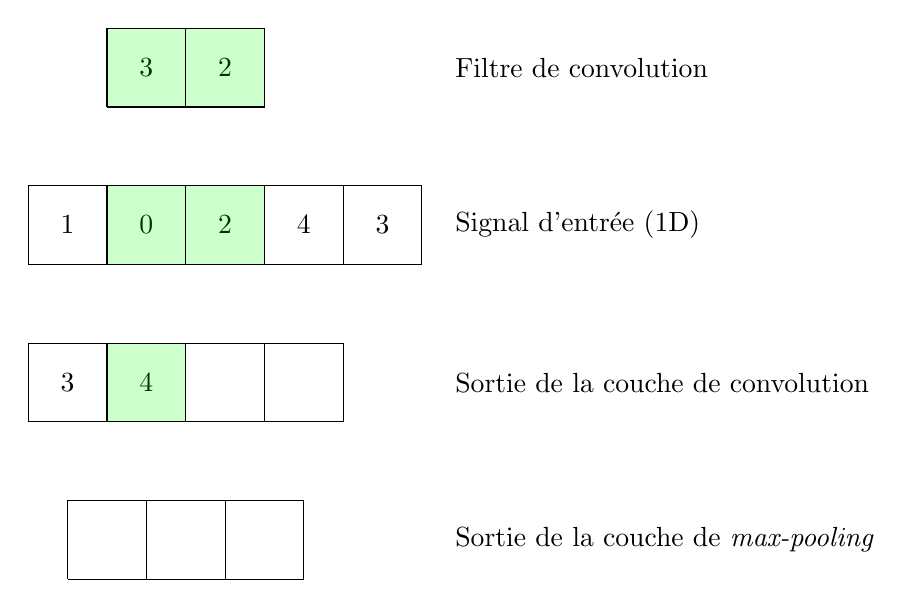
\begin{tikzpicture}

\node[anchor=west] (text0) at  (5.3,0.5) {Filtre de convolution};
\node[anchor=west] (text0) at  (5.3,-1.5) {Signal d'entrée (1D)};
\node[anchor=west] (text0) at  (5.3,-3.5) {Sortie de la couche de convolution};
\node[anchor=west] (text0) at  (5.3,-5.5) {Sortie de la couche de \emph{max-pooling}};
\node(filter_0_text) at (1.5, 0.5) {3};
\draw[fill=green, fill opacity=0.2] (1.0, 0.0) -- (2.0, 0.0) -- (2.0, 1.0)  -- (1.0, 1.0)  -- (1.0, 0.0);
-- cycle\node(filter_1_text) at (2.5, 0.5) {2};
\draw[fill=green, fill opacity=0.2] (2.0, 0.0) -- (3.0, 0.0) -- (3.0, 1.0)  -- (2.0, 1.0)  -- (2.0, 0.0);
-- cycle\node(input_0_text) at (0.5, -1.5) {1};
\draw (0.0, -2.0) -- (1.0, -2.0) -- (1.0, -1.0)  -- (0.0, -1.0)  -- (0.0, -2.0);
-- cycle\node(input_1_text) at (1.5, -1.5) {0};
\draw[fill=green, fill opacity=0.2] (1.0, -2.0) -- (2.0, -2.0) -- (2.0, -1.0)  -- (1.0, -1.0)  -- (1.0, -2.0);
-- cycle\node(input_2_text) at (2.5, -1.5) {2};
\draw[fill=green, fill opacity=0.2] (2.0, -2.0) -- (3.0, -2.0) -- (3.0, -1.0)  -- (2.0, -1.0)  -- (2.0, -2.0);
-- cycle\node(input_3_text) at (3.5, -1.5) {4};
\draw (3.0, -2.0) -- (4.0, -2.0) -- (4.0, -1.0)  -- (3.0, -1.0)  -- (3.0, -2.0);
-- cycle\node(input_4_text) at (4.5, -1.5) {3};
\draw (4.0, -2.0) -- (5.0, -2.0) -- (5.0, -1.0)  -- (4.0, -1.0)  -- (4.0, -2.0);
-- cycle\node(output_0_text) at (0.5, -3.5) {3};
\draw (0.0, -4.0) -- (1.0, -4.0) -- (1.0, -3.0)  -- (0.0, -3.0)  -- (0.0, -4.0);
-- cycle\node(output_1_text) at (1.5, -3.5) {4};
\draw[fill=green, fill opacity=0.2] (1.0, -4.0) -- (2.0, -4.0) -- (2.0, -3.0)  -- (1.0, -3.0)  -- (1.0, -4.0);
-- cycle\node(output_2_text) at (2.5, -3.5) {};
\draw (2.0, -4.0) -- (3.0, -4.0) -- (3.0, -3.0)  -- (2.0, -3.0)  -- (2.0, -4.0);
-- cycle\node(output_3_text) at (3.5, -3.5) {};
\draw (3.0, -4.0) -- (4.0, -4.0) -- (4.0, -3.0)  -- (3.0, -3.0)  -- (3.0, -4.0);
-- cycle\node(pool_0_text) at (1.0, -5.5) {};
\draw (0.5, -6.0) -- (1.5, -6.0) -- (1.5, -5.0)  -- (0.5, -5.0)  -- (0.5, -6.0);
-- cycle\node(pool_1_text) at (2.0, -5.5) {};
\draw (1.5, -6.0) -- (2.5, -6.0) -- (2.5, -5.0)  -- (1.5, -5.0)  -- (1.5, -6.0);
-- cycle\node(pool_2_text) at (3.0, -5.5) {};
\draw (2.5, -6.0) -- (3.5, -6.0) -- (3.5, -5.0)  -- (2.5, -5.0)  -- (2.5, -6.0);
-- cycle
\end{tikzpicture}

\end{document}
